\title{How Hard Are Your Negatives? A Pre-Registered Audit of Negative Ladders for Retrieval-Feature Abstention Gates, with a Negative Result}
\author{Shubh (PSIT, BCA)}
\date{}
\maketitle
\textit{Student author: Shubh (PSIT, BCA, first semester). Analysis and code: agent-assisted, human-directed (§7).}

\textit{Draft generated from \texttt{05\_paper/template/draft\_template.md} by \texttt{05\_paper/build\_draft.py}; every table}

\textit{below is written by \texttt{04\_experiments/src/make\_paper\_assets.py} from a results file, and every numeral is}

\textit{bound to \texttt{04\_experiments/RESULTS-INDEX.json}.}

\textit{Pre-registration: the pre-registration file in the experiments directory, whose three recorded hashes}

\textit{(frozen, then two amendments) cover the declared deviations D1--D3.}

\section{Abstract}
An abstention gate for retrieval-augmented question answering decides whether the retrieved passage

supports an answer. How hard such a gate looks depends on the negatives it is measured against, and we

tested that dependence with a pre-registered four-rung ladder over the SQuAD development set, fitting the gate and

both of its thresholds on a disjoint half. The result is negative and specific. The registered rule ---

maximise abstain recall subject to a dev abstain precision of

0.80 --- produced a gate that refuses

75.50\% of answerable questions, so it answers only

24.50\% of the questions it is asked, and the precision of

the items it refuses is 83.03\% pooled. At that

operating point the quantity the ladder was built to move stops moving: the per-rung refusal rate is

100.00\%,

99.64\%,

100.00\% and

100.00\% (H1 criterion not exercisable at this operating point, R1 minus R3 =

0.00\%, 95\% CI [0.00\%,

0.00\%]), a two-sided band is indistinguishable from the one-sided

threshold it was meant to beat (H3 criterion not exercisable at this operating point, difference 0.00\%, 95\% CI

[0.00\%, 0.00\%]), and dev-to-held-out

transfer is trivial rather than informative (H2 degenerate, loss

0.07\%). The audit that produced that verdict is the useful part. Six

surface features separate no rung from answerable items (AUROC

0.506, 0.539,

0.488, 0.415);

adding question--passage overlap to the same six features separates the first three almost perfectly

(0.977, 0.889,

0.923). The refusals are mostly answerable questions, which

is what an over-refusal of 75.50\% means: the band's

precision is

56.98\% on R1 and

48.02\% on R2. Overlap separates each rung from answerable items, and the exploratory refusal rates invert between R2 (91.07\%) and R3 (92.75\%), with the overlap-matched R5 (89.25\%) between them. Two control arms make that

concrete: an overlap-matched rung (R5, exploratory) is still refused at

\textit{89.25\%, while the rung that changes what the passage *says}

rather than how much of it overlaps (R4, one answer span replaced inside the gold passage) breaks the gate

once the dense features are implemented as specified --- refusal on R4 falls to

12.53\% and discrimination from

0.982 to 0.874 AUROC.

We report this as a negative result for the gate and a positive one for the audit: an abstention precision

is not interpretable without its coverage, and a negative-ladder result is not interpretable without an

overlap control.

\section{1 Introduction}
A retrieval-augmented system that always answers will sometimes answer from a passage that does not

support the question. An abstention gate is the component that decides, before generation, whether to

answer from the passage it was given. Gates are built from retrieval signals --- lexical scores, dense

cosine, reranker scores --- and they are evaluated against a set of negatives that is usually described in

one sentence.

That sentence matters. Abdumalikov et al. (arXiv:2403.01461) train on random negative excerpts, then

evaluate on excerpts with high semantic overlap, and report accuracy falling from

98\% to 1\%. A gate

measured only on random negatives would look finished. The honest reading of that result is not that

gates are bad; it is that the negative sampler, not the gate, was doing most of the work in the earlier

numbers.

So we designed a measurement rather than a method. One corpus (the SQuAD development set, arXiv:1806.03822), one

question set, one feature extractor, one fitting procedure, and four rungs of negatives that differ only

in how they were constructed. Three hypotheses were frozen before any result-producing run:

\begin{itemize}
  \item \textbf{H1 (hardness monotonicity).} Abstain precision is non-increasing across the rungs and falls by at
\end{itemize}
least fifteen points from R1 to R3.

\begin{itemize}
  \item \textbf{H2 (operating-point transfer).} The dev-fitted operating point loses at least ten points of abstain
\end{itemize}
precision at equal abstain recall when applied to a disjoint held-out half and to a second corpus.

\begin{itemize}
  \item \textbf{H3 (two-sided beats one-sided).} A two-threshold band beats the best single threshold on the same
\end{itemize}
score, by at least five points, at matched abstain recall.

The pre-registered analysis refutes H1 and H3 and leaves H2 degenerate, and we say so in the abstract

rather than in a footnote. That is the negative contribution, and it is the main one: at a precision

target without a coverage constraint, a gate can satisfy the target by refusing almost everything, and

when it does, the quantity the ladder is supposed to measure stops existing.

The instrument that made that negative result legible is itself the contribution:

\begin{itemize}
  \item \textbf{A reproducible four-rung ladder} over a closed public corpus, with item counts, drop rates and
\end{itemize}
construction code another lab can re-run (§3.1).

\begin{itemize}
  \item \textbf{A separability audit as a hard gate}, run before any result is reported: a classifier that sees
\end{itemize}
only surface properties of the text must not be able to tell a rung's negatives from answerable

items, or the rung is measuring formatting (§3.4, Table 2). Its sensitivity variant --- the same

features plus question--passage overlap --- is what turns the audit from a formatting check into a

measurement of what the rungs actually vary.

\begin{itemize}
  \item \textbf{A measurement of the coverage--precision pathology} in gate fitting: every refusal rate is reported
\end{itemize}
beside the precision of those refusals, the over-refusal that produced them and the coverage they leave,

with the observation that a two-sided band buys nothing when the admit region is degenerate (§4.2,

Table 4).

\begin{itemize}
  \item \textbf{Two control arms that localise the effect}: overlap-matched negatives (R5) and a top-1-presented
\end{itemize}
variant in which every item shows the retriever's first choice (§4.4, §4.5, Table 5). Together they

say what the gate is really measuring.

\begin{itemize}
  \item \textbf{An implementation correction, disclosed} (§4.6, Table 6): the frozen run's dense block was
\end{itemize}
degenerate because the presented passage was used as its own dense query. Re-implementing the

feature as specified lowers held-out AUROC and changes which rung is hard. We report both runs.

We claim neither priority nor generality beyond one corpus family, one feature stack, one gate family and

English passage-level question answering.

\section{2 Related work}
\textit{*Abstention and selective prediction.** Surveys of abstention in language models (arXiv:2407.18418)}

\textit{organise the space by what the model is uncertain about --- the query's answerability, the model's own}

\textit{confidence, or the values at stake --- and our gate addresses only the first of those. **Negative choice in}

\textit{answerability.** The collapse from near-perfect to near-zero accuracy when random-negative training is}

\textit{tested on high-overlap excerpts (arXiv:2403.01461) is the observation this paper is built on; our ladder}

\textit{is a systematic version of its two conditions. **Benchmarks that join retrieval and generation}

\textit{abstention.** DeclineCraft (arXiv:2610.28340) measures retrieval-side and parametric abstention jointly;}

\textit{our ladder varies only the presented passage and never asks the model to rely on memory, so the two}

\textit{designs are complementary rather than nested. \textbf{Retrieval components.} BM25 through the \texttt{bm25s}}

\textit{implementation; dense retrieval with a small BGE English model (arXiv:2309.07597); cross-encoder}

\textit{reranking in the passage-reranking tradition (arXiv:1901.04085) with the \texttt{ms-marco-MiniLM-L-6-v2}}

\textit{weights; dense passage retrieval as a baseline reference (arXiv:2004.04906). **Model confidence as a}

\textit{gate.** Eliciting a model's probability that a proposed answer is true (arXiv:2207.05221) is the}

\textit{strongest cheap reader-side baseline a reviewer expects; we ran a weaker reader signal --- mean}

\textit{generated-token log-probability --- and report why it failed here (§4.7). Table 1 sets the closest work}

\textit{beside this one on data, negatives, metric and reported operating point.}

\textit{*Table 1.** The closest work, compared on data, negative construction, metric and the operating point it reports. Literature comparison only: no experimental n, split or units beyond those each source reports.}

\begin{table}[t]
\centering
\scriptsize
  \begin{tabularx}{\textwidth}{lXXXX}
    \toprule
    Work & Data & Negatives & Metric & Operating point reported \\
\midrule
    Abdumalikov et al., arXiv:2403.01461 & ODQA corpora, SQuAD v2.0 pairs for repair & random text excerpts versus excerpts with high semantic overlap & answerability accuracy & one accuracy figure per sampler; coverage not reported \\
    DeclineCraft, arXiv:2610.28340 & retrieval and parametric abstention suite & several unanswerable classes & joint abstention metrics & per category, retrieval and memory reported separately \\
    This paper & SQuAD v2.0 dev, article-disjoint split & four constructed rungs, plus overlap-matched and top-1-presented variants & abstain precision, over-refusal, coverage & every precision reported with over-refusal and coverage beside it \\
    \bottomrule
  \end{tabularx}
\end{table}
\section{3 Method}
\subsection{3.1 Items}
SQuAD v2.0 dev (arXiv:1806.03822) contains

35 articles,

1204 paragraphs and

11873 questions, of which

5928 are answerable. Only the answerable rows are used;

impossible rows are a different kind of negative and are out of scope for this study. Articles are split

whole, never at paragraph level, into a dev half and a held-out half. From each half we sample four

hundred answerable questions and present each question with five passages, one per rung:

\begin{table}[t]
\centering
\scriptsize
  \begin{tabularx}{\textwidth}{lXX}
    \toprule
    Rung & Label & Presented passage \\
\midrule
    R0 & answerable & the question's gold paragraph \\
    R1 & negative & a uniformly sampled other paragraph from the same split's pool \\
    R2 & negative & a paragraph containing the question's highest-IDF content token \\
    R3 & negative & the paragraph immediately before or after the gold paragraph, in the same article \\
    R4 & negative & the gold paragraph with its first answer span replaced by a same-surface-type value \\
    \bottomrule
  \end{tabularx}
\end{table}
The ladder varies the negative in one \textit{respect} at a time --- unrelated text (R1), topically anchored text

(R2), adjacent text from the same document (R3), and text that is the gold passage except for one span

(R4) --- but not in only one respect: the rungs also differ in length and in provenance, which is why §4.4

and §4.6 use controls rather than assuming the rungs are otherwise matched. This yields 3752 items

(1879 held out); R2 is short at

273 dev items because most questions have no content word that

occurs in a paragraph other than their own. Following the pre-registration the rung is reported at its

true size rather than topped up, and §4.7 checks that the questions which kept an R2 item are not

different from those which did not.

\subsection{3.2 Features}
12 retrieval-side features per item: the BM25 score and

log-rank of the presented passage, corpus top-1 and mean-top-5 scores, the top-1/top-2 margin; the same

four for dense cosine; whether BM25 and dense agree on the top document; the cross-encoder score of the

presented passage; and question--passage token overlap. A rung-4 passage is a rewrite rather than a corpus

document, so it inherits its source paragraph's rank and is flagged.

\subsection{3.3 Gate and operating point}
A logistic regression on standardised features, fitted on dev only, gives a score that is meant to read

as the probability that the presented passage answers the question. Two operating points are fitted on

dev, both constrained to the observed dev score range: a band that admits only inside two thresholds, and

a single threshold that admits above one. Both maximise dev abstain recall subject to a dev abstain

precision of 0.80. The fitted band is

[0.9072, 0.9478], width

0.0406; the fitted single threshold is

0.9394. All three sit inside the observed dev score range, so the

failure this paper reports is not a threshold placed outside the data: it is that the admissible region

is degenerate. Dev admit mass is 6.03\%, and

92.95\% of dev items are refused by the lower threshold

alone.

\subsection{3.4 Separability audit}
Before any result is reported, a logistic regression on

6 surface features (characters, tokens, digit ratio,

upper-case ratio, punctuation ratio, mean word length) is fitted with

5-fold cross-validation, separately per rung, to tell that

rung's negatives from answerable items. Any rung above an AUROC of

0.750 is rebuilt by length-matched resampling, at most twice;

if two or more rungs still fail after a rebuild the run stops and the audit is the finding. A sensitivity

variant adds question--passage overlap and question length to the same features. It is labelled a

sensitivity variant, not a surface check, because overlap is a retrieval signal and calling it surface

would measure whether retrieval works rather than whether a rung leaks its identity through formatting.

The audit is one-sided by design: it flags a rung when surface features separate it from answerable items

in the expected direction, not when they separate it inverted. R4 comes out at

0.415, which is separation of the same magnitude with the

sign flipped, and is reported as that rather than as a clean pass.

\subsection{3.5 What the reported numbers are, and a correction to one name}
The pre-registration names two quantities and then gives one estimator. It calls the per-rung figure

abstain precision = P(negative | refused) and defines it as the mean of the refusal indicator over that

rung's negatives", which is P(refused | negative) --- a recall on that rung. Round-2 review caught the

contradiction, and it matters: at the registered operating point the per-rung refusal rate saturates at

100.00\% while the precision of those same refusals is between

48.02\% and

56.98\%, because three quarters of the answerable questions

are refused alongside the negatives. We therefore report both, always labelled: \textbf{refusal rate} for

P(refused | negative), which is the quantity H1 and H3 are stated over and the one the pre-registration

called abstain precision, and \textbf{precision} for P(negative | refused), computed over the rung's items and

the answerable items together. Pooled precision is

83.03\% at the registered point and

97.29\% at the exploratory point. No hypothesis is

restated over precision: the registered tests stay exactly as they were frozen, and the precision numbers

are descriptive.

\subsection{3.6 Statistics}
Item-level BCa bootstrap, 10000 resamples, seed

12345; paired comparisons resample items jointly; exact sign tests

for paired binary indicators; Holm correction over the two tests that carry p-values (H1 and H3; H2 has

none, because one side of it is the fitting half). Two intervals in §4.2 are zero-width because every item in that comparison is refused and every paired

difference is therefore zero; a zero-width interval at a boundary is reported as a boundary, not as

certainty. Rates are reported to two decimals and AUROC to three,

in line with the precision the intervals support. AUROC itself carries no interval: the bootstrap used

here intervals rates, not ranking statistics, and the change from one run to another is reported as a

difference between two analyses rather than as a tested contrast.

\section{4 Results}
\subsection{4.1 The audit passes, and says something uncomfortable}
\textit{*Table 2.** Separability audit on the dev half (1873 items): AUROC (unitless) of a logistic regression on six surface features, and the same features plus question--passage overlap, separating each rung's negatives from answerable items; gate 0.750; n per rung as listed in Table 3.}

\begin{table}[t]
\centering
\scriptsize
  \begin{tabularx}{\textwidth}{lXXX}
    \toprule
    Rung & Six surface features & + question--passage overlap & Gate \\
\midrule
    R1 & 0.506 & 0.977 & pass (gate 0.750) \\
    R2 & 0.539 & 0.889 & pass (gate 0.750) \\
    R3 & 0.488 & 0.923 & pass (gate 0.750) \\
    R4 & 0.415 & 0.408 & pass (gate 0.750) \\
    R5 (exploratory) & 0.721 & 0.794 & pass (gate 0.750) \\
    \bottomrule
  \end{tabularx}
\end{table}
On the six pre-registered surface features no rung is separable from answerable items, so the ladder is

not a formatting artefact and the run is allowed to proceed. Add question--passage overlap to the same six

features and R1 becomes almost perfectly identifiable:

0.977. That number is the paper's most transferable

single measurement. It says the rungs differ mainly in how much of the question the passage's words cover,

which is precisely what a lexical retriever scores, and it predicts the main result before the gate is

fitted. R4 is the exception: overlap does not identify it

(0.408), because R4's passage \textit{is} the gold passage.

\subsection{4.2 At the pre-registered operating point the ladder disappears}
\textit{*Table 3.** Held-out results per rung (held-out half, 1879 items; n per rung as listed): refusal rate P(refused | negative) and precision P(negative | refused), percent; both the band and exploratory operating points.}

\begin{table}[t]
\centering
\scriptsize
  \begin{tabularx}{\textwidth}{lXXXXX}
    \toprule
    Rung & n & Band refusal rate & Band precision & Exploratory refusal rate & Exploratory precision \\
\midrule
    R1 & 400 & 100.00\% & 56.98\% & 99.75\% & 91.30\% \\
    R2 & 280 & 99.64\% & 48.02\% & 91.07\% & 87.03\% \\
    R3 & 400 & 100.00\% & 56.98\% & 92.75\% & 90.71\% \\
    R4 & 399 & 100.00\% & 56.92\% & 84.71\% & 89.89\% \\
    \bottomrule
  \end{tabularx}
\end{table}
Refusal rate is P(refused | a negative of that rung) --- a recall on the rung, and the quantity the pre-registration labelled abstain precision. Precision is P(negative of that rung | refused), over that rung's items and the answerable items together. Pooled precision is 83.03\% at the registered point and 97.29\% at the exploratory point; the band gate answers 24.50\% of answerable questions, while its item-level coverage is much lower because every question contributes four negatives to the item count.

\textit{*Table 4.** The three pre-registered hypotheses, their criteria, observed values and verdicts (held-out half; percentages).}

\begin{table}[t]
\centering
\scriptsize
  \begin{tabularx}{\textwidth}{lXXX}
    \toprule
    Hypothesis & Pre-registered criterion & Observed & Verdict \\
\midrule
    H1 hardness monotonicity & R1 - R3 at least 15 points, non-increasing & difference 0.00\%, 95\% CI [0.00\%, 0.00\%]; sequence is not non-increasing & REFUTED \\
    H2 transfer & loss at least 10 points; refuted if within 5 points & dev-to-test loss 0.07\% & REFUTED (it transfers, degenerately) \\
    H3 two-sided vs one-sided & band at least 5 points ahead at matched recall & difference 0.00\%, 95\% CI [0.00\%, 0.00\%] & REFUTED \\
    \bottomrule
  \end{tabularx}
\end{table}
Table 3 reports the refusal rate and the precision of those refusals per rung, for both operating points.

The band refuses 100.00\%,

99.64\%,

100.00\% and

100.00\% of the four rungs' negatives, refuses

75.50\% of answerable questions, and therefore answers

24.50\% of the questions it is asked. Three verdicts follow,

and none of them is the one the design was hoping for.

\begin{figure}[t]
  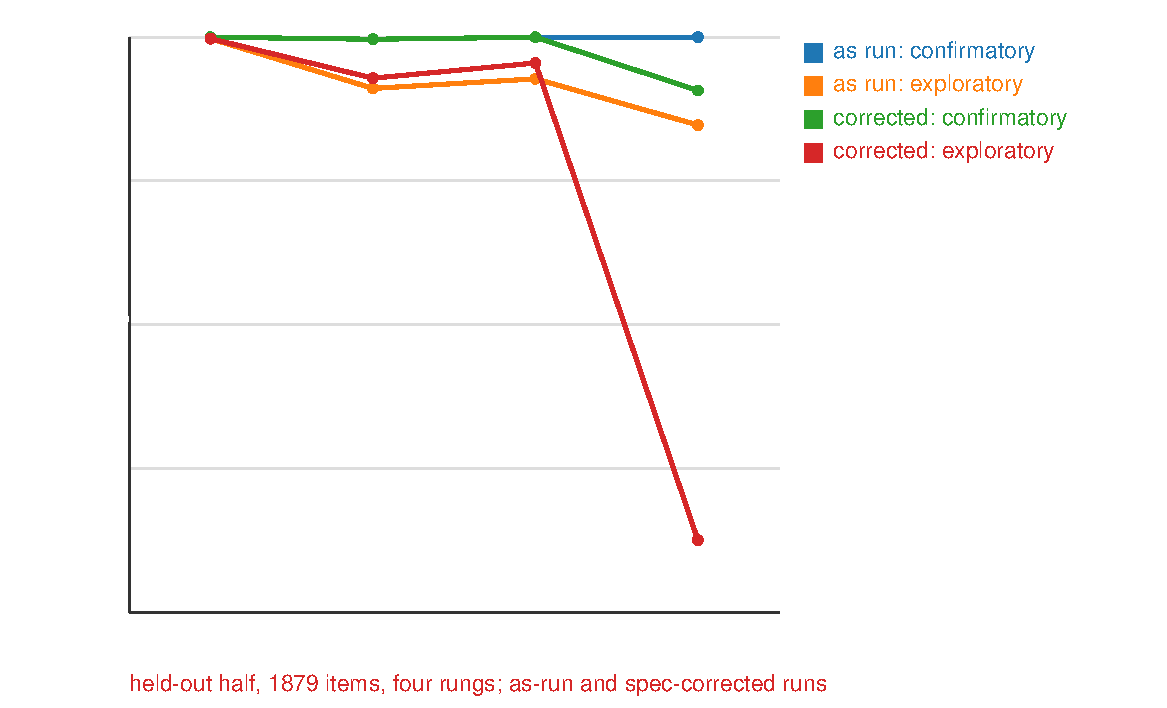
\includegraphics[width=0.85\linewidth]{figures/F1_abstain_precision_by_rung.pdf}
  \caption{Held-out results across the four rungs for both runs.}
  \label{fig:main-accuracy}
\end{figure}
and plots the same quantities across the four rungs for both runs; the flat as-run curves and the collapsed

corrected R4 are visible in it directly.

\begin{figure}[t]
  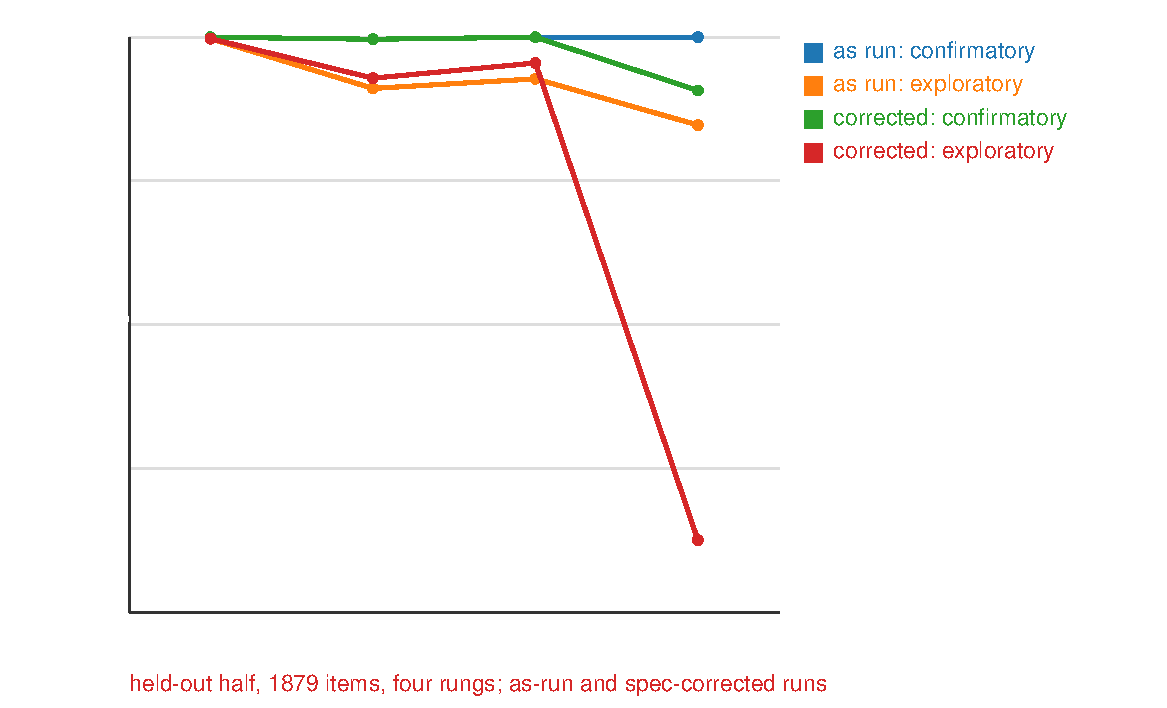
\includegraphics[width=0.85\linewidth]{figures/F1_abstain_precision_by_rung.pdf}
  \caption{Held-out results across the four rungs for both runs.}
  \label{fig:main-accuracy}
\end{figure}
\textit{Figure 1. Abstain precision (\%) by rung (R1--R4) for the as-run confirmatory and exploratory bands and the}

\textit{spec-corrected confirmatory and exploratory bands, on the held-out half (1879 items); flat as-run curves}

\textit{and the collapsed corrected R4 are visible directly.}

\begin{figure}[t]
  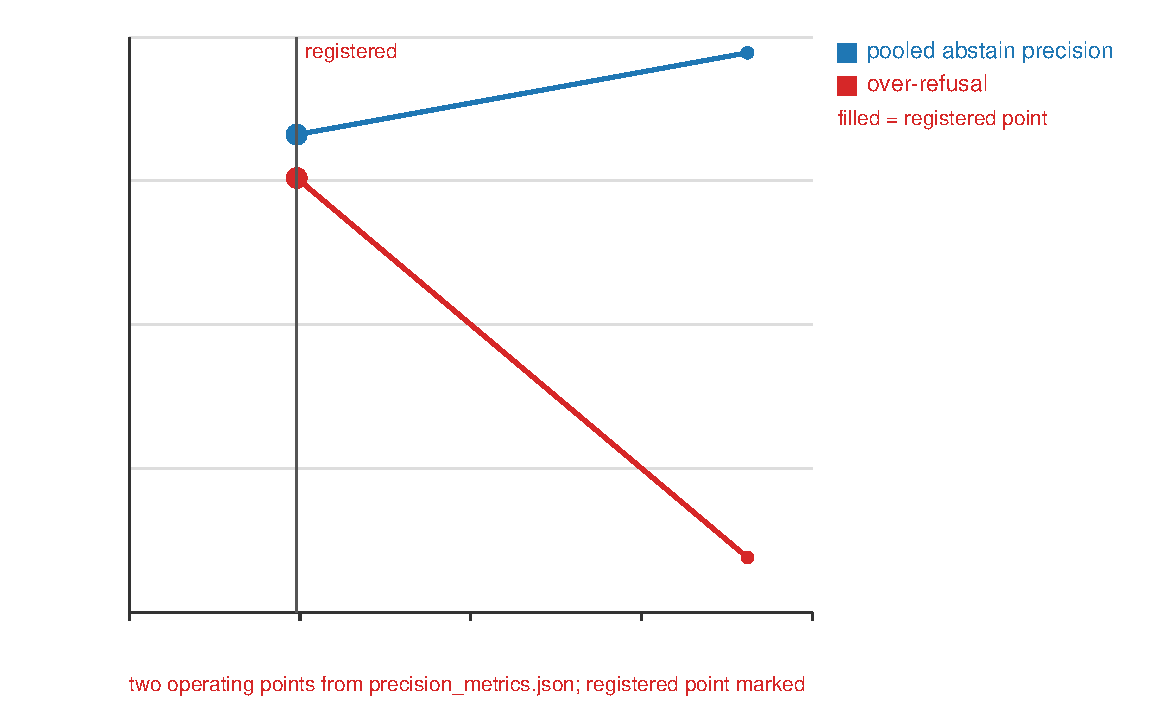
\includegraphics[width=0.85\linewidth]{figures/F2_precision_overrefusal_vs_coverage.pdf}
  \caption{Held-out results across the four rungs for both runs.}
  \label{fig:main-accuracy}
\end{figure}
\textit{Figure 2. Pooled abstain precision (\%) and over-refusal (\%) against coverage (questions answered / questions asked,}

\textit{held-out half, 1879 items) for the two registered operating points; the confirmatory band}

\textit{(coverage 24.50\%, pooled precision 83.03\%,}

\textit{over-refusal 75.50\%) and the exploratory band (coverage}

\textit{25.44\%, pooled precision 97.29\%,}

\textit{over-refusal 9.50\%) are shown; the registered operating point is marked.}

\textit{*H1: criterion not exercisable at this operating point.** R1 minus R3 is 0.00\% with a 95\% CI of}

\textit{[0.00\%, 0.00\%]; the sequence is not}

\textit{non-increasing and the fifteen-point criterion is not met. Strictly, this is a criterion not met at an}

\textit{operating point that makes the quantity uninformative, and the two readings differ: the criterion is}

\textit{not exercisable at this operating point, the mechanism it was meant to test is not. The exploratory operating point shows a 7.00\% drop (R1 to R3), reported beside this verdict. §4.3 moves the operating point and finds the effect at}

\textit{about half the predicted size, which is why we do not read the refutation as evidence that negative}

\textit{hardness does not matter.}

\textit{*H3: criterion not exercisable at this operating point.** At the band's dev recall the recall-matched single threshold gives an identical}

\textit{held-out refusal rate: the difference is 0.00\% with a 95\% CI of}

\textit{[0.00\%, 0.00\%]. The band and the}

\textit{matched single threshold refuse the same negatives to within}

\textit{0.00 points in every rung, and the band's only measurable}

\textit{effect is worse over-refusal: 75.50\% against}

\textit{72.50\%. Two-sidedness buys nothing when almost everything}

\textit{is refused on the low side. The reason is structural: the recall-matched single threshold is the band's own}

\textit{lower threshold to five decimal places, so the upper threshold never binds and the two gates are the same}

\textit{gate. That degeneracy is the finding, not a flaw in the comparison.}

\textit{*H2 is degenerate rather than supported.** Dev pooled precision is essentially identical to held-out}

\textit{pooled precision, a loss of 0.07\%, which the pre-registered rule counts}

\textit{as refuted-in-the-direction-that-means-it-transfers. A gate that refuses}

\textit{92.95\% of dev items on its lower threshold alone cannot}

\textit{fail to transfer. This is robustness of the trivial kind and we do not present it as stability.}

The precision figures show what those refusals contain:

56.98\% of the band's refusals on R1 and

48.02\% on R2 are that rung's negatives, so most of what the

gate refuses with such a high pre-registered precision is an answerable question. Dev precision at the

fitted band is 83.69\%, so the rule did exactly what it was

asked; what it was asked was not enough.

The two single-score baselines show what the gate is doing. A threshold on BM25 top-1 pooled abstain

precision of 1.69\%: it can only buy precision by refusing nothing

useful. A dense-cosine score reaches 74.58\% pooled --- but in this

run that score is constant, so the figure is an artefact of a degenerate column rather than a baseline,

which is the defect §4.6 corrects.

\subsection{4.3 Exploratory: constrain coverage and the ladder returns, partly}
The registered rule is not the rule a practitioner would use, so before its numbers existed we declared a

second operating point (deviation D1): maximise dev recall subject to precision

0.80 and dev over-refusal at most

0.10. It keeps over-refusal at

9.50\% with coverage

25.44\%, and the per-rung refusal rate now falls across the

ladder:

99.75\%,

91.07\%,

92.75\%,

84.71\%, while the precision of those refusals stays

between 87.03\% and

91.30\% in every rung. The R1 to R3 drop is

7.00\% with a paired-by-question 95\% CI of

[4.50\%, 9.75\%] --- real, but

half the pre-registered fifteen-point criterion, and not monotone (R2 sits below R3). R1 to R4 is

15.04\%, CI [11.53\%,

18.80\%]. So the ladder is not invisible; it is bought out by

coverage at the registered point, and at a coverage-constrained point it appears at about half the

predicted size. This is exploratory, it rescues no hypothesis, and the confirmatory verdict stands.

\subsection{4.4 Control arm: matching the overlap does not defeat the gate}
If the rungs differ from answerable items chiefly in question--passage overlap, then a negative built to

match the gold paragraph's overlap should be the hardest possible negative for an overlap-driven gate. We

built it (deviation D2): for each sampled question, the candidate paragraph whose overlap with the

question is closest to the gold paragraph's overlap. Matching is as good as the pool allows rather than

exact --- the mean absolute overlap difference is

10.29\% on the held-out half, against

42.08\% for a random negative, so R5 is closer to the gold

paragraph's overlap than any other rung.

\textit{*Table 5.** Control arms (all exploratory): refusal rates, 95\% CI, over-refusal and discrimination (held-out half; percentages; AUROC unitless). Precision is reported for the main ladder only (Table 3).}

\begin{table}[t]
\centering
\scriptsize
  \begin{tabularx}{\textwidth}{lXXXX}
    \toprule
    Arm (all exploratory) & Abstain precision & 95\% CI & Over-refusal & Discrimination \\
\midrule
    Rung R5, confirmatory band & 100.00\% & [100.00\%, 100.00\%] & degenerate, see §4.4 & 0.974 \\
    Rung R5, exploratory band & 89.25\% & [85.75\%, 91.75\%] & matching residue 10.29\% & 0.974 \\
    Second-corpus arm, confirmatory band & 98.50\% & not informative & 89.50\% & 0.640 \\
    Second-corpus arm, exploratory band & 85.50\% & [79.50\%, 89.50\%] & 57.50\% & 0.640 \\
    Top-1 presented (hit rate 78.25\%) & 87.30\% P(miss & refused) & not informative & 2.56\% of hits refused \\
    \bottomrule
  \end{tabularx}
\end{table}
Every arm here is exploratory. R5 and the top-1 variant are declared deviations (D2, D3). The second-corpus arm is H2's pre-declared second corpus, but its construct differs (no article grouping, shorter passages, multi-hop questions), so it supports a direction claim only.

The gate is not defeated: R5's negatives are refused at

89.25\% (95\% CI

[85.75\%, 91.75\%]) at the

exploratory point, which places it between R2 (91.07\%) and

R4 (84.71\%) in the ordering. Overlap is therefore not the whole story: R5

items also differ in length (they are the longest negatives in the ladder), and the surface audit is

closest to its gate on this rung (0.721 on dev) without

crossing it. The honest reading is that a paragraph drawn from elsewhere in the corpus can be caught by

several correlated signals, and matching one of them is not enough to hide it.

All numbers in this subsection come from the as-run gate. The spec-corrected gate is at least as strict on

this arm, so the arm's conclusion does not depend on the dense defect reported in §4.6.

\subsection{4.5 Control arm: what the gate does when the passage is always the retrieved one}
The first review round's top objection was that answerable items always present the gold paragraph while

negatives never do, so the gate may be reading is this the document retrieval found rather than

answerability. The pre-registered design cannot answer that, so we built the variant (deviation D3): every

item presents the BM25 rank-1 paragraph for its question, labelled answerable if that paragraph is the

gold paragraph. The retriever's first choice is correct for

78.25\% of held-out questions, so this variant has a real mixture

of hits and misses rather than a constant label.

The same feature stack detects retrieval correctness at

0.945 AUROC on the held-out half, refuses

63.22\% of retrieval misses and

2.56\% of retrieval hits, and when it refuses, the passage is

usually a miss (P(miss refused) = 87.30\%). That is a good

retrieval-correctness detector. It is also the reason the ladder result should be read carefully: in this

variant the label \textit{is} retrieval correctness, so detects misses and detects unanswerable passages

coincide item for item, and the comparison cannot separate the two readings. It confirms the mechanism

the audit implies and it does not exculpate the gate.

\subsection{4.6 The dense block was degenerate: a disclosed implementation correction}
Two readers of the code, working separately, found the same defect, and it changes the numbers. In the

frozen implementation the dense query was the presented passage itself rather than the question, so

\texttt{dense\_presented} and \texttt{dense\_top1} were identical to each other, the dense cosine was exactly one on

78.70\% of as-run rows (every row of R0--R3, none of R4), and

\texttt{dense\_rank\_log} was constant;

the two dense columns also received the same fitted coefficient. The gate therefore had ten informative

columns, not twelve, and the dense-cosine baseline in §4.2 was a constant score.

We did not refit the registered analysis: the frozen run is reported exactly as it was produced. Instead

we implemented the feature as §3.2 specifies --- a question-to-passage cosine --- and re-ran the whole

analysis through the same code path as a declared sensitivity analysis (deviation D4). Table 6 puts the

two side by side, and Table 7 reports leave-one-group-out ablations on the corrected features.

\textit{*Table 6.** The pre-registered (frozen, D1) run versus the spec-corrected re-implementation (D4), side by side (dev and held-out halves; AUROC unitless, rates percent). The two runs refit their thresholds on different dev score distributions, so precision and coverage rows compare two operating points; AUROC rows are threshold-free.}

\begin{table}[t]
\centering
\scriptsize
  \begin{tabularx}{\textwidth}{lXX}
    \toprule
    Quantity & Frozen run & Spec-corrected (D4) \\
\midrule
    Gate AUROC, dev & 0.988 & 0.887 \\
    Gate AUROC, held out & 0.982 & 0.874 \\
    Band lower threshold (t\_lo) & 0.9072 & 0.5232 \\
    Band upper threshold (t\_hi) & 0.9478 & 0.5370 \\
    Band abstain precision, R1 & 100.00\% & 100.00\% \\
    Band abstain precision, R2 & 99.64\% & 99.64\% \\
    Band abstain precision, R3 & 100.00\% & 100.00\% \\
    Band abstain precision, R4 & 100.00\% & 90.73\% \\
    Band over-refusal & 75.50\% & 91.50\% \\
    Band coverage & 5.27\% & 3.83\% \\
    Exploratory precision, R1 & 99.75\% & 99.75\% \\
    Exploratory precision, R2 & 91.07\% & 92.86\% \\
    Exploratory precision, R3 & 92.75\% & 95.50\% \\
    Exploratory precision, R4 & 84.71\% & 12.53\% \\
    Exploratory over-refusal & 9.50\% & 11.00\% \\
    Exploratory coverage & 25.44\% & 39.60\% \\
    H3 band minus matched single & 0.00\% & -2.23\% \\
    Dense-cosine (B2) pooled precision & 74.58\% & 99.73\% \\
    Dense-cosine (B2) coverage & 27.73\% & 0.27\% \\
    \bottomrule
  \end{tabularx}
\end{table}
\textit{*Table 7.** Leave-one-group-out ablations on the spec-corrected features, with the same threshold rule refitted for each subset (dev and held-out halves; n = features retained; AUROC unitless; rates percent).}

\begin{table}[t]
\centering
\scriptsize
  \begin{tabularx}{\textwidth}{lXXXXX}
    \toprule
    Feature subset & n & Dev AUROC & Held-out AUROC & Band over-refusal & Exploratory R4 \\
\midrule
    all\_12 & 12 & 0.887 & 0.874 & 91.50\% & 12.53\% \\
    dense\_only & 4 & 0.888 & 0.870 & 94.75\% & 23.06\% \\
    lex\_overlap\_only & 1 & 0.812 & 0.811 & 92.25\% & 10.03\% \\
    no\_bm25 & 7 & 0.881 & 0.868 & 91.25\% & 12.53\% \\
    no\_cross\_encoder & 11 & 0.886 & 0.872 & 93.75\% & 13.78\% \\
    no\_dense & 8 & 0.867 & 0.862 & 87.75\% & 9.77\% \\
    no\_lex\_overlap & 11 & 0.888 & 0.874 & 90.50\% & 13.03\% \\
    no\_rank & 10 & 0.884 & 0.872 & 92.25\% & 13.28\% \\
    \bottomrule
  \end{tabularx}
\end{table}
Three things change and one does not. Held-out AUROC falls from

0.982 to 0.874: the

frozen figure was flattered by a column that encoded this passage is a corpus document rather than this

passage answers the question. The exploratory ladder changes shape: R1 to R3 stay in the nineties

(99.75\%,

92.86\%,

95.50\%) and R4 collapses to

12.53\%. R4 is the rung whose passage is the gold

passage with one span swapped, so a feature set that scores how well a passage matches a question has

nothing to work with: the passage matches perfectly and the answer is wrong. That is the failure mode the

gate should have, and the frozen run hid it because the degenerate dense column was in effect a

presented-versus-gold flag. The confirmatory verdicts do not change: H1 remains refuted

(0.00\%), H2 remains degenerate, and H3 remains refuted --- now in

the stronger form that the band is worse than the recall-matched single by

-2.23\% (95\% CI

[-3.11\%, -1.35\%]).

Two caveats on that last number: the matched single threshold is refitted on corrected dev scores, where

its dev precision falls below the 0.80 constraint, so the

comparison is descriptive rather than a re-run of the registered test; and the corrected exploratory band

ends at an over-refusal of 11.00\%, above the

0.10 cap it was constrained to on dev

--- the constraint is on dev, not on the held-out half, and we report the breach rather than hide it.

The corrected dense baseline is a real score at a degenerate operating point:

99.73\% pooled precision at

0.27\% coverage.

No single group carries the corrected result in these point estimates --- removing any one group costs less

than a third of the AUROC margin --- but eight point estimates without intervals cannot establish

equivalence, and we do not claim it. What Table 7 does show is the size of each group's contribution:

removing the dense group costs

0.862 held-out AUROC against

0.874 for the full set, and overlap alone reaches

0.811. No single group carries the result; the

separation is distributed across overlap, BM25 and dense scores, which is what one expects when all of

them measure the same thing.

\subsection{4.7 Robustness of the pieces the ladder rests on}
Four checks a reviewer asked for, all of them cheap and all of them reported as they came out.

\textit{*Is the short rung a biased subsample?** Of the four hundred sampled questions per split,}

\textit{273 kept an R2 item and}

\textit{127 did not. Comparing the two groups on question length,}

\textit{answer surface type, gold paragraph length and article size, no variable differs at the five-percent level in}

\textit{either split; the smallest p-value is 0.052, on dev question}

\textit{length. So the R2 figures describe the sampled question set rather than a selected subset, with the caveat}

\textit{that several p-values sit between five and ten percent.}

\textit{*Do the intervals survive clustering?** Resampling whole articles instead of items leaves every verdict}

\textit{unchanged. Of the five comparable cells, four cluster intervals are narrower than the item intervals (narrowest:}

\textit{confirmatory R2, width ratio 0.45) and one is slightly}

\textit{wider (exploratory R4, 1.17), because the refusal rate is}

\textit{almost constant across the held-out articles and there is almost no article-level variance for clustering}

\textit{to add. Two cells are}

\textit{zero-width at both levels because every item in them is refused.}

\textit{*Is the matched-recall comparison fair?** The recall-matched single threshold is chosen on dev, never on}

\textit{test. On the held-out negatives the band and the matched single refuse the same items to within}

\textit{0.00 points, with zero discordant pairs, so H3's zero is not a}

\textit{binning artefact.}

\textit{*Does the reader-confidence baseline work?** No, and for an inspectable reason. On the}

\textit{553 dev items where it was run (a small instruction-tuned reader,}

\textit{mean generated-token log-probability), the signal reaches AUROC}

\textit{0.419 --- worse than chance. When the reader refuses it emits a}

\textit{fixed refusal string at near-certainty, so a correct refusal scores as high confidence and a confident}

\textit{wrong answer scores low. Mean log-probability measures the fluency of the string produced, not evidential}

\textit{support. We report the baseline as exploratory and do not use it to rank gates.}

\subsection{4.8 Second corpus: direction only}
The lower rows of Table 5 are the second-corpus arm. Scored against the registered rule, the arm's exploratory loss is neither the ten-point failure nor

inside the plus-or-minus-five-point refutation band; the pre-registration defines no verdict for a

five-to-ten-point loss, so H2's second arm is recorded as \textbf{inconclusive by the registered rule} rather

than claimed as either.

The pre-declared second corpus (the multi-hop corpus described in §3.1 of the pre-registration;

400 items built, half answerable and half drawn from the

same question's non-supporting article pool) is evaluated with the frozen operating point. At the

confirmatory point the arm reports 98.50\% precision at an

over-refusal of 89.50\%, which is the same degeneracy as the

main corpus and therefore uninformative; at the exploratory point it reports

85.50\% (95\% CI [79.50\%,

89.50\%]), a drop of

7.25 points against the main corpus's R3. Discrimination, however,

falls from 0.982 on the main corpus to

0.640 on this one. The construct differs --- no article grouping,

shorter passages, multi-hop and comparison questions --- so we read this as a direction claim only: transfer

of the \textit{operating point} survives, transfer of the \textit{discrimination} does not, and a paper that reported

only the precision number would have said the opposite.

\section{5 Discussion}
\subsection{5.1 A precision target without a coverage constraint is not a specification}
The registered rule --- maximise recall subject to precision of

0.80 --- is the rule a practitioner writes down, and it

produced a gate that answers about one question in four

(24.50\% of answerable questions) and whose refusals are

only 83.03\% true negatives. Any paper reporting

abstention performance without over-refusal and coverage beside it should be read as reporting a choice

about how often to refuse. Our

own 75.50\% over-refusal is the number that makes the

precision figure interpretable, and it belongs first, not in a limitations paragraph.

\subsection{5.2 What a retrieval-feature gate measures}
The audit, the overlap-matched rung and the top-1 variant agree on one description: these features

measure how well the presented passage matches the question and how likely it is to be the document

retrieval wanted. On negatives constructed by substituting paragraphs, those quantities and answerability

move together, which is why the ladder looks like a hardness ladder. When they come apart --- R4, where the

passage matches perfectly and one span is wrong --- the gate has nothing to work with, and the corrected run

shows it. The practical implication is not that abstention gates are useless. It is that a ladder of

substituted paragraphs measures overlap, and that the rung which changes what the passage says must be in

the ladder or the ladder is measuring the wrong thing.

\subsection{5.3 Why the corrected run matters more than the frozen one}
We report the frozen analysis as the registered result and the corrected analysis as a deviation, but a

reader should treat the corrected numbers as the ones worth carrying forward. The frozen gate's

discrimination was inflated by a column that encoded a construction artefact, and its R4 behaviour was

the opposite of what the construct implies. Reporting both, with the defect in the text, is the only

honest option available after the fact; the alternative --- quietly refitting and calling it the result ---

would have been exactly the move this paper is about.

\subsection{5.4 What would make the ladder a stronger instrument}
Three changes, in order of expected value. Present, for every item, the passage the retriever actually

returns rather than the gold passage for answerables: that is what §4.5 approximates, and it should

replace the current R0 instead of being an add-on. Build R4 by hand rather than by type-matched

substitution: forty inspected rung-4 items included substitutions that preserved the surface type but not

the grammatical role, which weakens the premise-violation reading to answer-absent. And evaluate at a

declared coverage, not a declared precision, so that the operating point cannot be satisfied by refusing

everything.

\section{6 Threats to validity}
1. One corpus family, one language, passage-level question answering, one feature stack, one gate family.

Nothing here is evidence about chapter-level or multi-hop retrieval.

2. The item construction presents the gold paragraph for answerable items, so part of the gate's

discrimination measures whether retrieval found the gold paragraph. §4.5 quantifies that component

rather than arguing about it.

3. R2 is incomplete (273 dev items and

280 held-out items against four hundred sampled questions), which

weakens any conclusion that depends on R2 specifically; §4.7 reports the exchangeability check.

4. R4 substitutions are automatic and sometimes ungrammatical.

5. The second-corpus arm is a direction test with a different construct, and its confirmatory operating

point is degenerate by construction.

6. The reader baseline covers 553 dev items only.

7. The gate is fitted on a dev half of 1873 items; intervals reflect

item-level and article-level resampling, not corpus-level uncertainty.

8. The frozen run's dense block was degenerate and the corrected re-implementation changes two of the

reported quantities (§4.6). Both runs are reported; neither is a substitute for a fresh pre-registered

replication with the corrected features.

\section{7 Ethics, data and AI disclosure}
Public data only: SQuAD v2.0 dev (share-alike licence) and the multi-hop corpus dev split (Apache licence, as declared by

the authors' repository), with every request logged with URL, status, size and checksum in

\texttt{04\_experiments/data/TRANSFER-DATA.md} and the per-request log files beside it. No private data, no scraped data, no login-walled source. The student is the

responsible author; code, seeds and raw outputs are committed beside the scripts that produced them (for example

\texttt{04\_experiments/src/gate.py}), and the pre-registration hash is recorded before the first

result-producing run.

AI assistance is disclosed per the target venue's policy. Language-model agents wrote analysis code,

ran the experiments, drafted sections and performed the simulated review; the simulated review is

labelled as a simulation and is not a venue decision. The student directed the work, holds the author

position, and is expected to be able to explain every section --- \texttt{06\_review/STUDENT-DIGEST-S3.md} exists to

make that possible, and \texttt{06\_review/CLAIMS-AUDIT.md} maps each claim to the file that supports it.

\section{8 Reproduction}
\begin{footnotesize}
\begin{verbatim}
python 04_experiments/src/build_items.py            # items, seeds fixed
python 04_experiments/src/features.py               # as-run features (dense block degenerate)
python 04_experiments/src/run_c1.py                 # the pre-registered analysis
python 04_experiments/src/features_corrected.py     # spec-corrected features (D4)
python 04_experiments/src/eval_corrected.py         # the corrected analysis
python 04_experiments/src/build_items_rung5.py && python 04_experiments/src/features_rung5.py \
  && python 04_experiments/src/eval_rung5.py        # R5 control arm
python 04_experiments/src/features_transfer.py && python 04_experiments/src/eval_transfer.py
python 04_experiments/src/build_items_top1.py && python 04_experiments/src/features_top1.py \
  && python 04_experiments/src/eval_top1.py         # top-1 control arm
python 04_experiments/src/ablation_corrected.py     # Table 7
python 04_experiments/src/stats_addendum.py         # §4.7 numbers
python 04_experiments/src/build_transfer_items.py  # the second-corpus items (§4.8)
python 04_experiments/src/reader_logprob.py        # the reader baseline (§4.7, dev only)
python 04_experiments/src/precision_metrics.py     # the refusal/precision split (Table 3)
python 04_experiments/src/make_paper_assets.py      # tables + index entries
python 05_paper/build_draft.py                      # this file, from the template
python tools/check_numbers.py --draft 05_paper/draft/paper.md
\end{verbatim}
\end{footnotesize}
The frozen run records its pre-registration hash as a single \texttt{\#} character: the line that reads the hash

file splits on whitespace and takes the first token of a comment line. The four real hashes are intact in

\texttt{PREREGISTRATION.sha256}, and this is a defect in the reporting line, not in the freeze.

There is no lockfile. The interpreter and library versions used for every number above are recorded in the

session status file beside the results, and the model versions are pinned in the pre-registration; a

requirements file with exact pins is the obvious next step and is not in this draft.


\bibliographystyle{plainnat}
\bibliography{refs}

